\documentclass{article}
\title{Labolatorium 1 - Sprawozdanie}
\date{28-04-2019}
\author{Filip Cinik 131734}

\usepackage{listings}
\usepackage{color}
\usepackage[T1]{fontenc}
\usepackage[polish]{babel}
\usepackage[utf8]{inputenc}
\usepackage{graphicx}

\definecolor{dkgreen}{rgb}{0,0.6,0}
\definecolor{gray}{rgb}{0.5,0.5,0.5}
\definecolor{mauve}{rgb}{0.58,0,0.82}

\lstset{frame=tb,
  language={[x86masm]Assembler},
  aboveskip=3mm,
  belowskip=3mm,
  showstringspaces=false,
  columns=flexible,
  basicstyle={\small\ttfamily},
  numbers=none,
  numberstyle=\tiny\color{gray},
  keywordstyle=\color{blue},
  commentstyle=\color{dkgreen},
  stringstyle=\color{mauve},
  breaklines=true,
  breakatwhitespace=true,
  tabsize=3
}

\begin{document}
\maketitle
\tableofcontents
\newpage

\section{Zadanie 1}
\subsection{Dodawanie szesnastkowe}
Program dodaje niższe bity stałej \textbf{Stala} do rejestru  \textbf{A} a następnie dodaje wyższe bity z przeniesieniem.

\begin{figure}[!htb]
  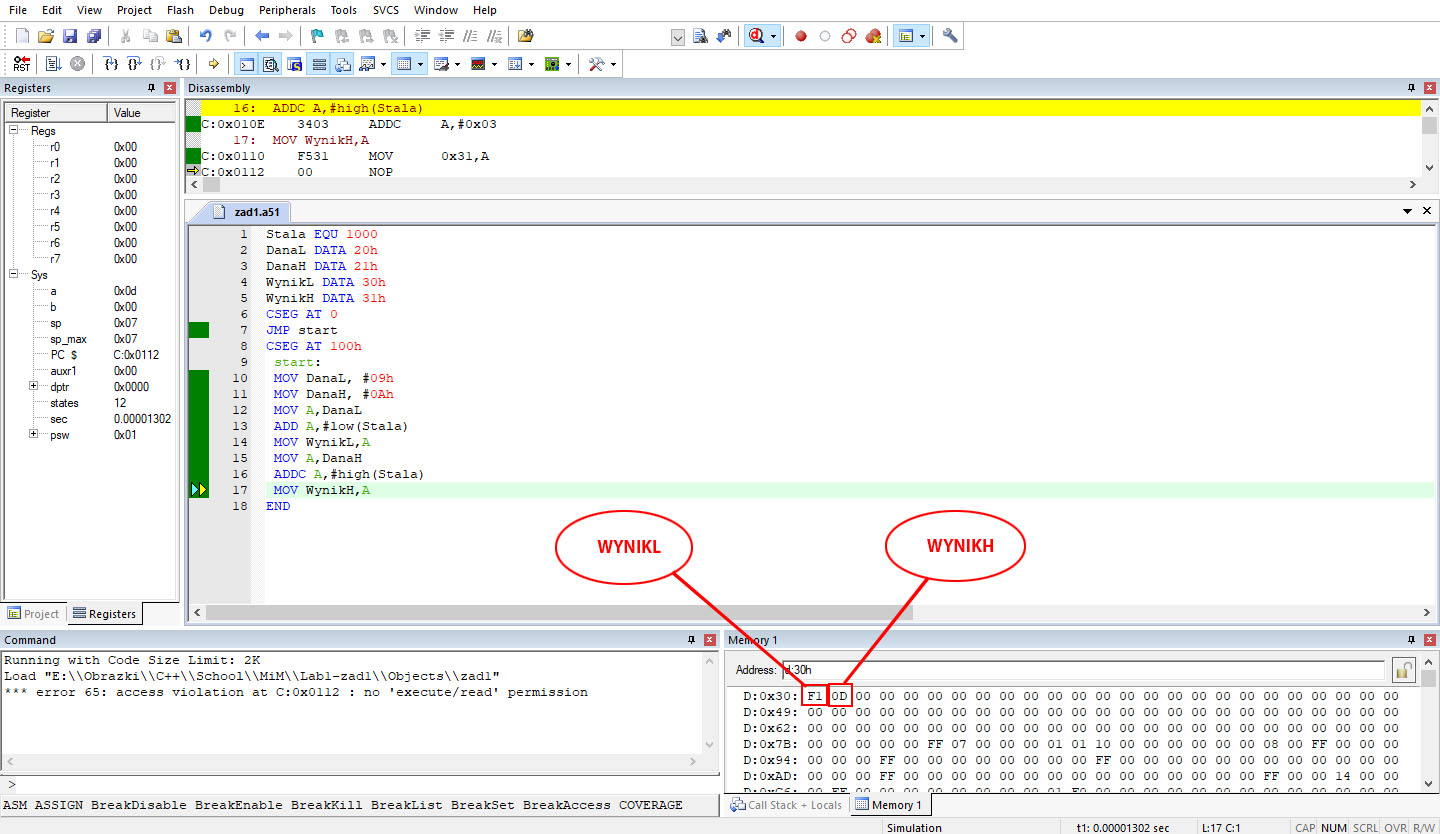
\includegraphics[width=\linewidth]{Fig2.jpg}
  \caption{Debug programu}
  \label{fig:fig2}
\end{figure}

Do manipulacji 16 bitowymi liczbami używa się poleceń \textbf{\#low} i \textbf{\#high}. Dzięki temu liczbę 16 bitową, nie mieszczącą się w całości w rejestrze, można zamienić na dwie liczby 8 bitowe i manipulować nimi osobno.

\subsection{Przepełnienie}

Kiedy do rejestru \textbf{A} dodane zostaną wartości większe od 255, następuje przepełnienie, który sygnalizowane jest poprzez ustawienie flagi \textbf{CY} na 1. Przepełnienie powoduje "zawinięcie się" liczby.

\begin{figure}[!htb]
  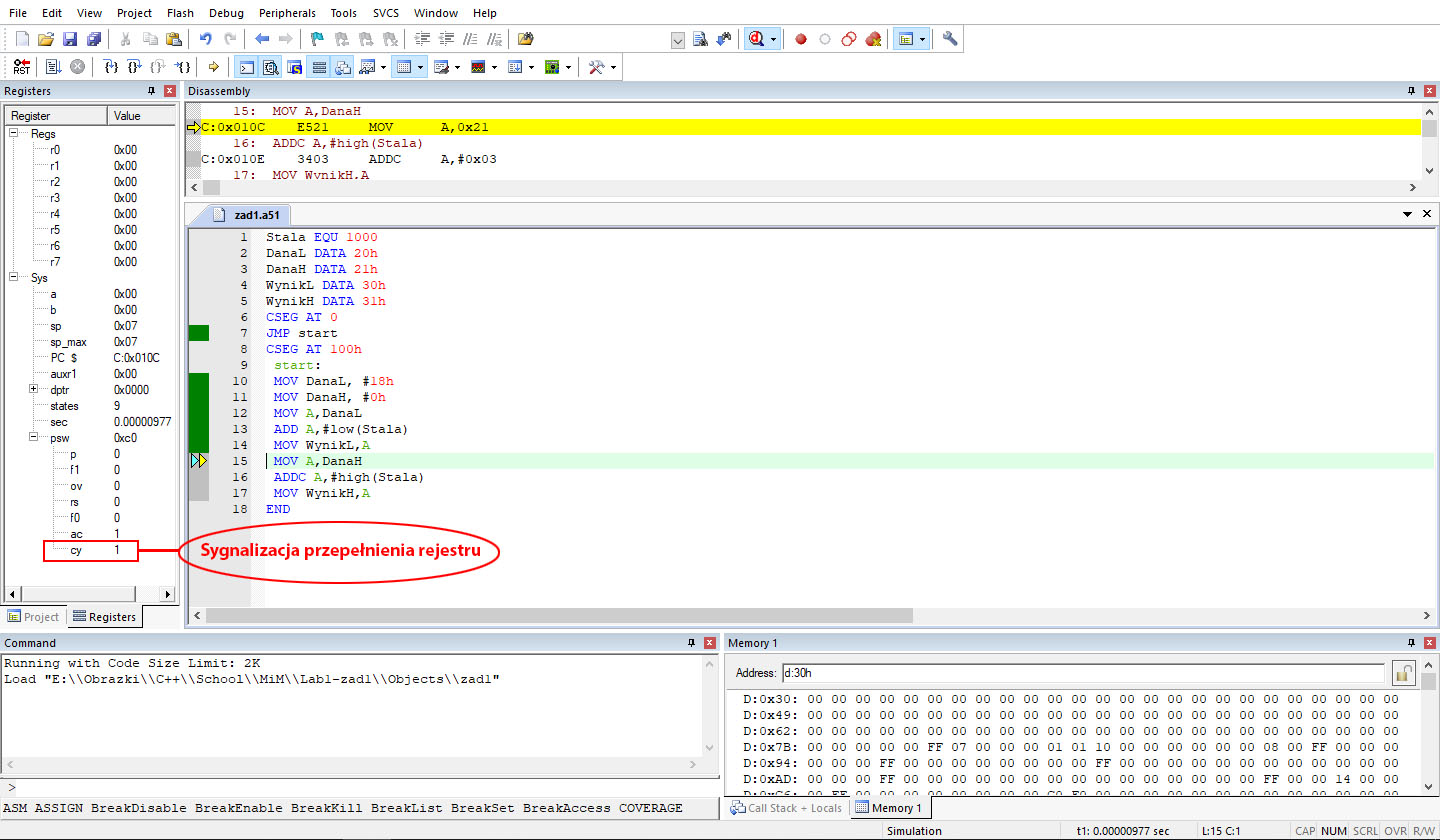
\includegraphics[width=\linewidth]{Fig3.jpg}
  \caption{Przepełnienie rejestru A}
  \label{fig:fig3}
\end{figure}

\newpage

\subsection{Odejmowanie}

Odejmowanie liczb z użyciem \textbf{SUBB}. Od 16 bitowej liczby \#FFFF odejmujemy niższe bity stałej \textbf{Stala} i zapisujemy je do \textbf{WynikL}, a następnie odejmujemy wyższe bity stałej \textbf{Stala} i zapisujemy je do \textbf{WynikH}.

\begin{figure}[!htb]
  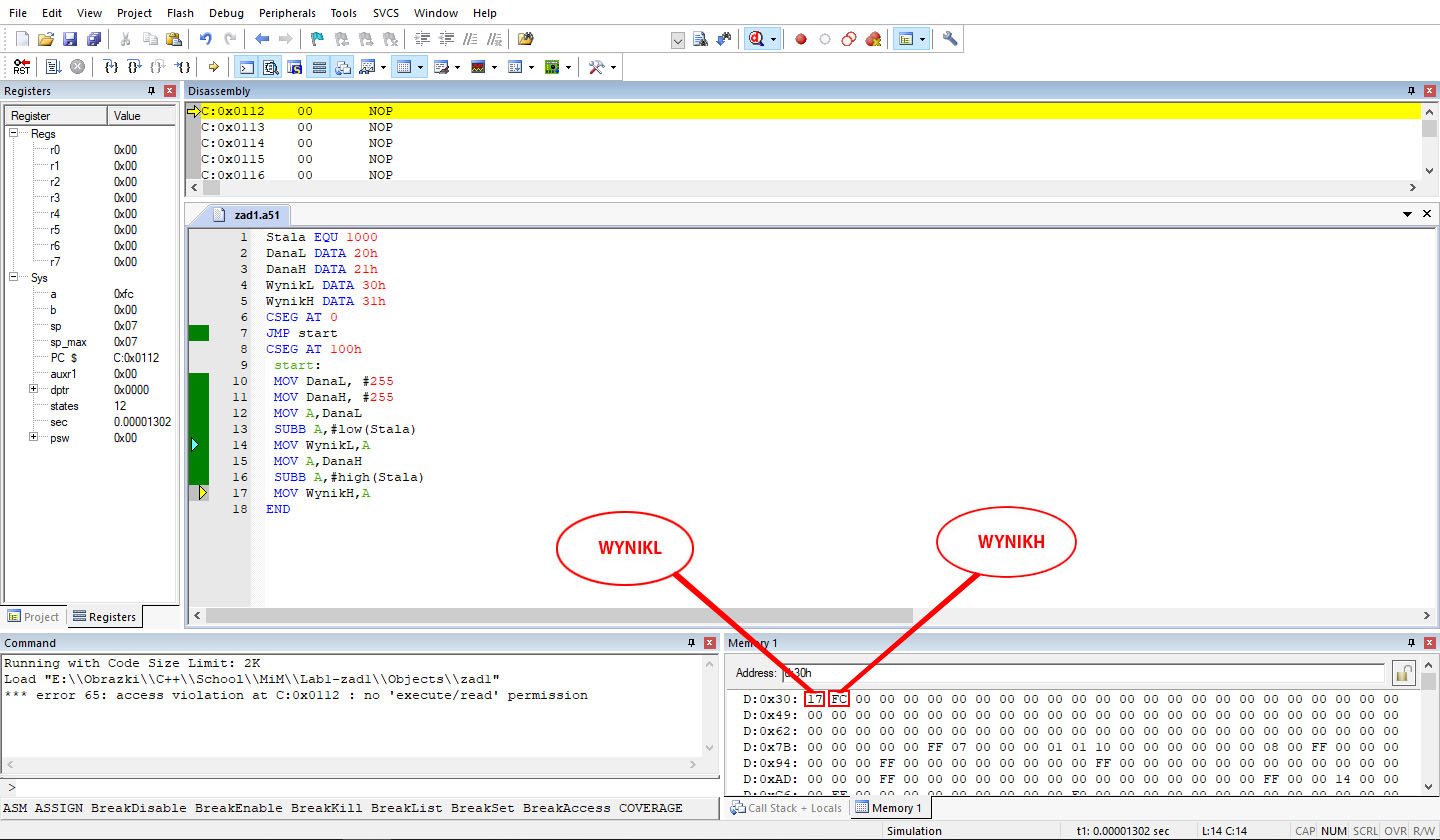
\includegraphics[width=\linewidth]{Fig4.jpg}
  \caption{Odejmowanie liczb}
  \label{fig:fig4}
\end{figure}

Wynik odjętych liczb widać powyżej. W przypadku odjęcia większej liczby od mniejszej, również dostatniemy przepełnienie, które zostanie zasygnalizowane poprzez ustawienie flagi \textbf{CY}.

\newpage



\section{Zadanie 3 - Generator liczb losowych}

Generator liczb losowych został zrealizowany poprzez użycie buforu \textbf{Buffer} przetrzymującego sekwencje 10 elementów w pamięci. Początkowo są używane liczby podane w treści zadania, które następnie są zastępowane przez kolejne wartości generowanej sekwencji pseudo-losowych liczb. Procedura \textbf{init} odpowiada za inicjalizację tych danych.

Wzór użyty do wygenerowania pseudo-losowej sekwencji liczb to ALFG - Addytywny Opóźniony Generator Fibonacciego (ang. \textit{Additive Lagged Fibonacci Generator})

$x_n=(x_{n+j}+x_{n+k}) * \bmod{m}$

$j = 7,$
$k = 10$

Gdzie $j$, $k$ i $n$ odpowiadają \textbf{J}, \textbf{K}, \textbf{N} w kodzie programu.

\section{Schemat działania}

Program uruchamia się w nieskończonej pętli wywołując procedurę \textbf{random}, która umieszcza nową liczbę pseudolosową w rejestrze \textbf{A} oraz zapisuję ją do buforu \textbf{Buffer}.

Procedura \textbf{random} w pierwszej kolejności upewnia się, że zmienne \textbf{J}, \textbf{K}, \textbf{N} są w zakresie 0-9 poprzez użycie reszty z dzielenia. Dzięki temu upewnia się, że nie przekroczyliśmy zakresu buforu. Następnie umieszcza w rejestrach \textbf{R0} i \textbf{R1} wartości \textbf{J} i \textbf{K}. Odbywa się to poprzez dodanie do adresu buforu offsetu, który wskaże na pozycje danej zmiennej w buforze.

Wartości z rejestrów \textbf{R0} i \textbf{R1} są sumowane aby otrzymać pierwszą część równania $(x_{n+j}+x_{n+k})$. Następnie liczone jest modulo poprzez umieszczenie wyniku dodawania w rejestrze \textbf{A} oraz liczby \textbf{4} w rejestrze \textbf{B} co daje nam drugą część równania $\bmod{m}$.

Ostatnim krokiem jest znalezienie pozycji zmiennej \textbf{N} w buforze poprzez, tak jak poprzednio, dodanie do adresu buforu wartości \textbf{N}, która jest jakby aktualnym indeksem naszej tablicy \textbf{Buffer}.

Nowa liczba pseudo-losowa jest przeniesiona do rejestru \textbf{A}, a wartości \textbf{J}, \textbf{K}, \textbf{N} są inkrementowane o 1.

\begin{center}
\begin{tabular}{ |c|c|c|c|c|c|c|c|c|c|c|c|c|c| } 
 \hline
	t & j & k & n & \multicolumn{10}{|c|}{Sekwencja} \\
 \hline
	0 & 6 & 9 & 0 & 4 & 5 & 3 & 3 & 3 & 4 & 6 & 2 & 6 & 5 \\ 
 \hline
	1 & 8 & 1 & 1 & \textbf{3} & 5 & 3 & 3 & 3 & 4 & 6 & 2 & 6 & 5 \\ 
 \hline
	2& 1 & 4 & 2  & 3 & \textbf{3} & 3 & 3 & 3 & 4 & 6 & 2 & 6 & 5 \\ 
 \hline
	3 & 5 & 8 & 3 & 3 & 3 & \textbf{2} & 3 & 3 & 4 & 6 & 2 & 6 & 5 \\ 
 \hline
	4 & 0 & 3 & 4 & 3 & 3 & 2 & \textbf{2} & 3 & 4 & 6 & 2 & 6 & 5 \\ 
 \hline
\end{tabular}
\end{center}

Powyżej zademonstrowano 5 pierwszych cykli generacji liczb. \textbf{J} i \textbf{K} zawijają się po przekroczeniu rozmiaru buforu.

\begin{figure}
  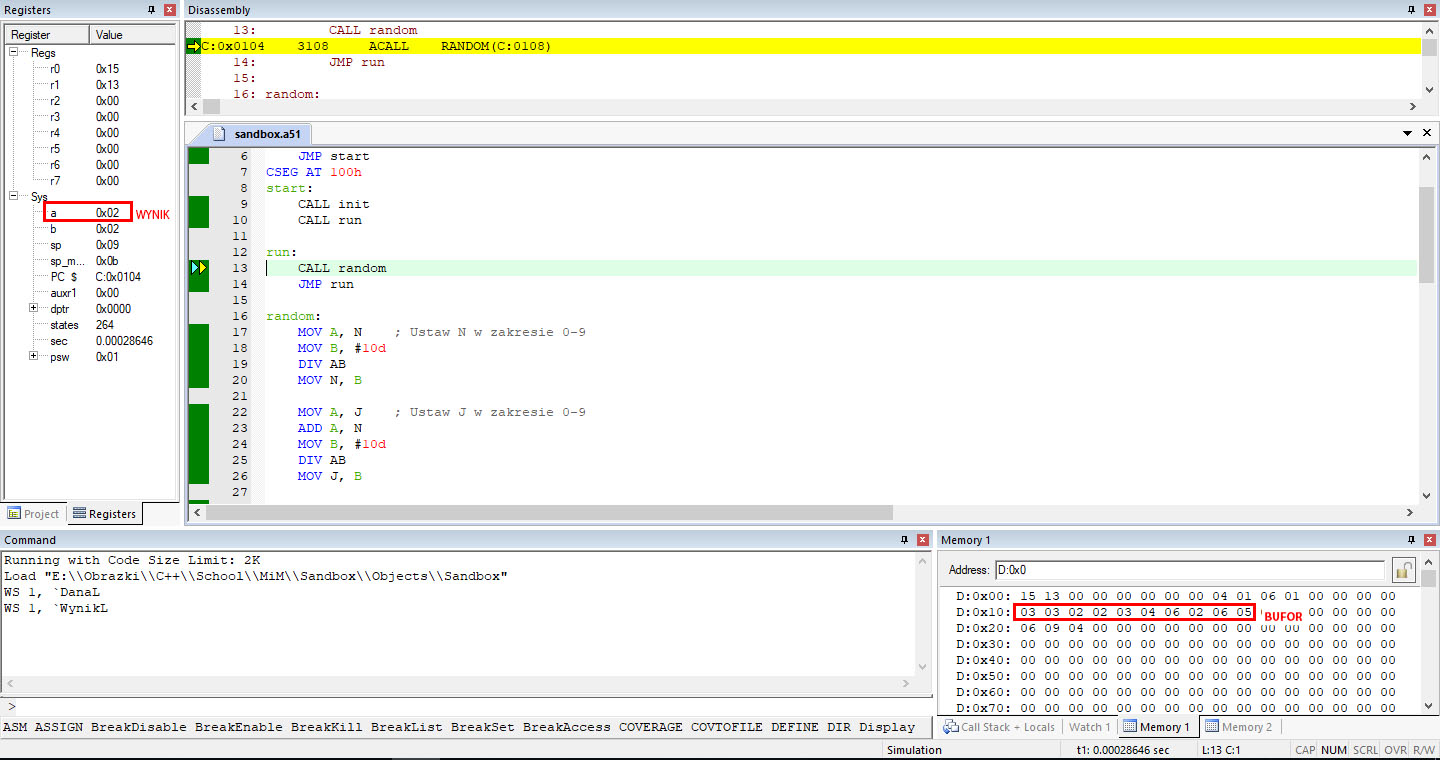
\includegraphics[width=\linewidth]{Fig1.jpg}
  \caption{Najważniejsze elementy pamięci}
  \label{fig:fig1}
\end{figure}


\section{Kod}

\begin{lstlisting}
Buffer DATA 10h
J DATA 20h
K DATA 21h
N DATA 22h
CSEG AT 0
	JMP start
CSEG AT 100h
start:
	CALL init
	CALL run

run:
	CALL random
	JMP run

random:	
	MOV A, N	; Ustaw N w zakresie 0-9
	MOV B, #10d
	DIV AB
	MOV N, B

	MOV A, J	; Ustaw J w zakresie 0-9
	ADD A, N
	MOV B, #10d
	DIV AB
	MOV J, B
	
	MOV A, K	; Ustaw K w zakresie 0-9
	ADD A, N
	MOV B, #10d
	DIV AB
	MOV K, B
	
	MOV A, #Buffer	; Wez wartosc Buffer + offset
	ADD A, J
	MOV R0, A
	
	MOV A, #Buffer	; Wez wartosc Buffer + offset
	ADD A, K
	MOV R1, A

	MOV A, @R0	; Buffer + J
	ADD A, @R1	; A + (Buffer + K)
	MOV B, #4d
	DIV AB		; Ustaw nowa liczbe w zakresie 0-3
	
	MOV A, #Buffer
	ADD A, N
	MOV R1, A
	MOV @R1, B
	
	MOV A, B	; Ustaw nowa wartosc w pozycji Buffer(n)
	
	INC J
	INC K
	INC N
	RET
 
init:
	MOV J, #6d
	MOV K, #9d
	MOV Buffer + 0, #4d
	MOV Buffer + 1, #5d
	MOV Buffer + 2, #3d
	MOV Buffer + 3, #3d
	MOV Buffer + 4, #3d
	MOV Buffer + 5, #4d
	MOV Buffer + 6, #6d
	MOV Buffer + 7, #2d
	MOV Buffer + 8, #6d
	MOV Buffer + 9, #5d
	RET
	
END
\end{lstlisting}

\end{document}